
\documentclass[runningheads,a4paper]{llncs}
\usepackage[margin=0.5in]{geometry}
\usepackage{amssymb}
\setcounter{tocdepth}{3}
\usepackage{graphicx}
\usepackage{amssymb}% http://ctan.org/pkg/amssymb
\usepackage{pifont}% http://ctan.org/pkg/pifont
\newcommand{\cmark}{\ding{51}}%
\newcommand{\xmark}{\ding{55}}%

\usepackage{floatrow}
% Table float box with bottom caption, box width adjusted to content
\newfloatcommand{capbtabbox}{table}[][\FBwidth]
\usepackage{caption}
\usepackage{subcaption}
\captionsetup{compatibility=false}

\usepackage{url} % for bibliograpy links
\urlstyle{same}  % (for bibliography links
\usepackage{float} % To force image to stand still

\usepackage{amsmath,amssymb}

\usepackage{color}

\usepackage{array}
\newcolumntype{P}[1]{>{\centering\arraybackslash}p{#1}}

\newcommand{\keywords}[1]{\par\addvspace\baselineskip
\noindent\keywordname\enspace\ignorespaces#1}

\begin{document}
\vspace{-100pt}
\mainmatter

\title{A Stochastic Approach to Optimization of Deterministic Finite Automata}

\titlerunning{Algorithms and Computability}

\author{Jakub Ciecierski \and Bartlomiej Dybisz \\ 
\textit{Warsaw University of Technology,\\
Faculty of Mathematics and Information Science.}}

\authorrunning{Algorithms and Computability}


\toctitle{Algorithms and Computability}
\tocauthor{Methodology}

\maketitle

%---------------------------------------------------------------------

\section{Model}

\begin{figure}[H]
	\centering
	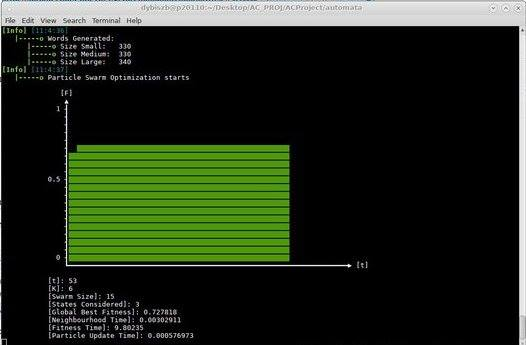
\includegraphics[width=0.4\textwidth]{images/console.jpg}
    \caption{Example of console}
    \label{fig:clustering_class}
\end{figure}


%---------------------------------------------------------------------
%---------------------------------------------------------------------
\subsection{Algorithm}\label{sec:algorithm}

%---------------------------------------------------------------
%---------------------------------------------------------------
\subsection{Clustering}

The clustering module contains all necessary functionality for analysis of clusters. Figure~\ref{fig:clustering_class} presents few basic classes. \textit{KMeans} constructor takes the maximum iterations and tolerance of convergence. Calling \textit{compute} will start the computation of kmeans algorithm with $k$ clusters for input data set. The private methods of KMeans are responsible for computing the corresponding sections of kmeans algorithm. It is important to note that \textit{initCentroids()} method could be implemented using many different algorithms, which might change the time complexity of kmeans algorithm and a whole.

Further, in figure~\ref{fig:clustering_class} sub module \textit{Evaluation} is presented. The class \textit{ClusterEvaluator} is a base class for all cluster evaluation algorithms. It consists of \textit{clustering tool} which shall be used to compute the optimal number of clusters for given data set. The \textit{compute} method will start looking for optimal $k$ from the interval $[start_k, end_k]$. At this stage of research, only McClain-Rao algorithm is proposed. In the future, if the need arises, further cluster evaluators should be derived from the base class \textit{ClusterEvaluator}.

%
% CLUSTERING CLASS DIAGRAM
%
\begin{figure}[H]
	\centering
	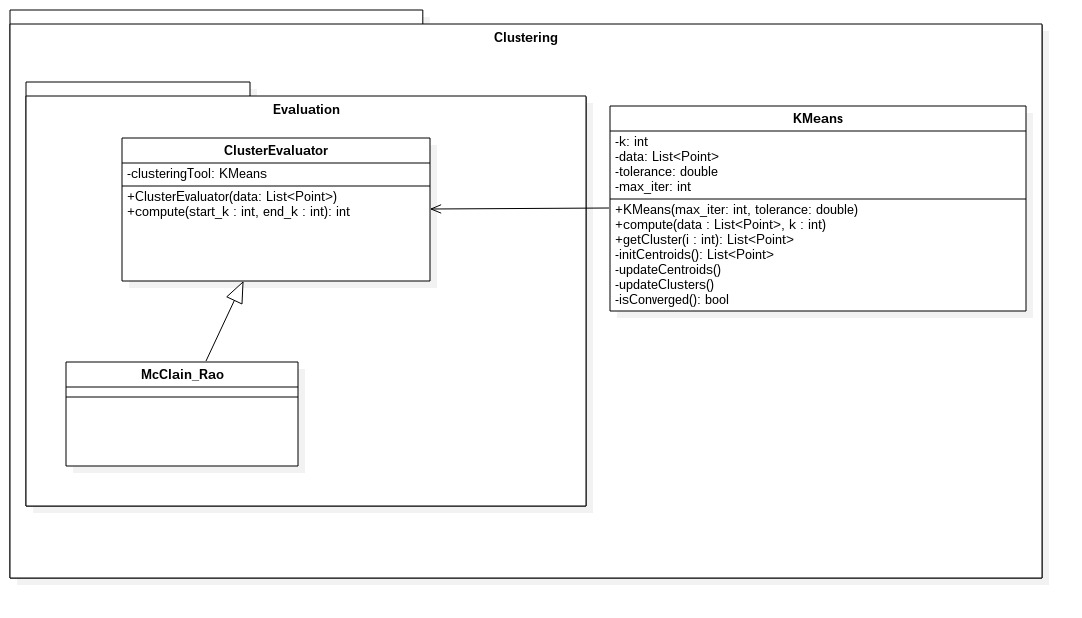
\includegraphics[width=0.4\textwidth]{images/clustering_class.jpg}
    \caption{Class diagrams of clustering module}
    \label{fig:clustering_class}
\end{figure}


%---------------------------------------------------------------
%---------------------------------------------------------------

\subsection{Classification}

The classification module deals with the problems of classifying objects. Figure~\ref{fig:classification_class} shows the appropriate module. The \textit{Classifier} class contains a word generator. Note that the word generator itself, might correspond to real or synthetic data generation. The Classifier will then look for automaton which will classify these words in the best manner possible. The method of finding such automaton is the PSO algorithm. The \textit{PSO} class encapsulates the Particle Swarm Optimization algorithm. As arguments it takes the number of states and number of symbols in the alphabet, which will govern the swarm size and the dimensions of particles. Note that \textit{\_bestParticles} field is a list, since there can exist many best solution. Thus the \textit{getResults} shall return all such results and the Classifier class should be responsible for picking the most appropriate one.

Lastly the \textit{Particle} class simply encapsulates the particle used in PSO.

%
% CLASSIFICATION CLASS DIAGRAM
%
\begin{figure}[H]
	\centering
	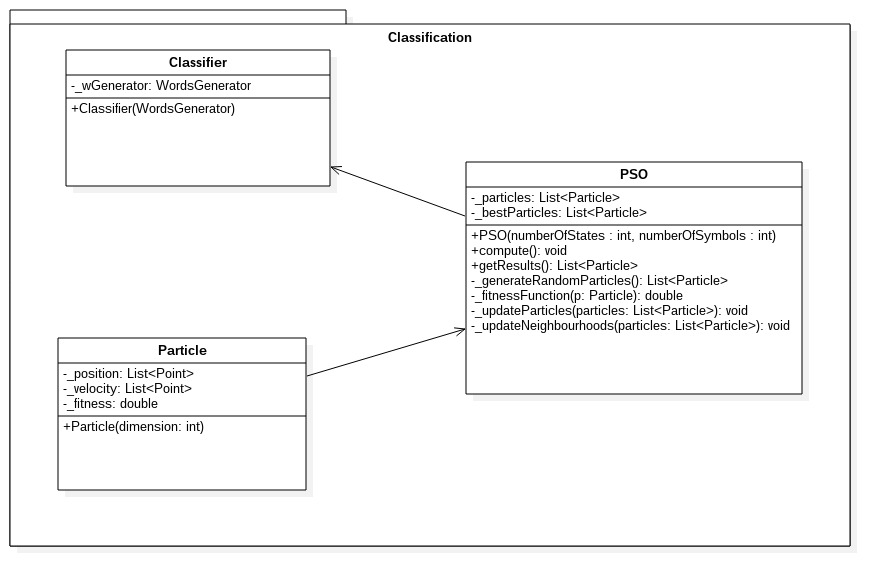
\includegraphics[width=0.4\textwidth]{images/classification_class.jpg}
    \caption{Class diagrams of classification module}
    \label{fig:classification_class}
\end{figure}



%---------------------------------------------------------------
%---------------------------------------------------------------
\subsection{Utility}

The utility module is presented in figure~\ref{fig:utility_class}. \textit{Logger} class is responsible for printing and saving logs of the computations. It contains path to log directory and a path to specific file in which the logs should be saved. The one parameter method \textit{log}, prints the message to default file. The two parameter \textit{log} is used when the message should be saved in a different file.

The \textit{Console} class is responsible for loading flag parameters from the console, and updating the global settings. The global settings, containing all parameters of the computations are stored in \textit{Settings} class.

Finally a simple clock mechanism is proposed in \textit{Clock} class. The \textit{startClock} method starts measuring time until \textit{stopClock} is called which returns the time taken between both methods' calls. The time is encapsulated in \textit{TimeStamp} class.


%
% UTILITY CLASS DIAGRAM
%
\begin{figure}[H]
	\centering
	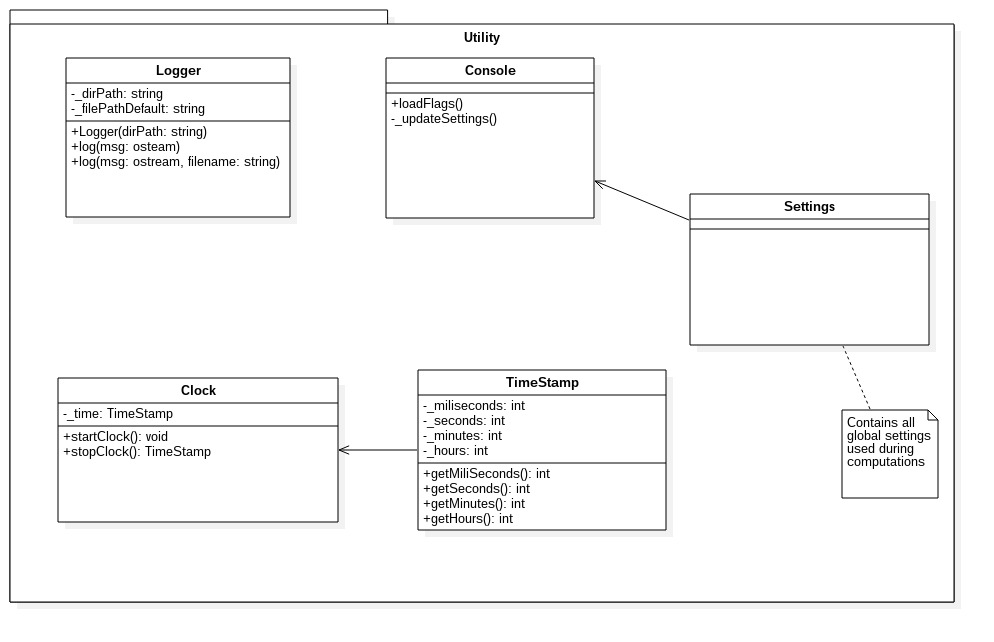
\includegraphics[width=0.4\textwidth]{images/utility_class.jpg}
    \caption{Class diagrams of utility module}
    \label{fig:utility_class}
\end{figure}




%---- BD ----%

%
% DFA CLASS DIAGRAM
%
\subsection{Deterministic Final Automaton}
In some sense this is most important class in the whole project. It represents automaton and its classical functionalities. Although class seems short, it uses objects of more sophisticated classes described in the subsections \ref{subsec:transition_table} and \ref{subsec:words_proc}. 

To start with we will describe fields of the class. \texttt{alphabet} is a vector of integers, which holds all symbols considered by automaton. It can be extracted from transition table using \texttt{\_acquireAlphabetFromTransitionTable()} method. Next and last one is \texttt{\_codedTransitionTable} object. In most general sense, object of this class mimics usage of transition table by allowing user to access and modify entries (see section \ref{sec:autom}), as well as coding and decoding table to form described in section \ref{sec:auto_dec}. 

Next we will look closer at constructors. First one generates random automaton based on provided number of states and alphabet. Alphabet takes values from interval [1,numberOfSymbols], hence it can be represented by single value: \texttt{numberOfSymbols}. Second constructor is suited to work with particle class. It reconstruct itself regarding to provided coded transition table, which in fact represents particle position. 

At the end a little bit about provided methods. \texttt{\_acquireAlphabetFromTransitionTable()} has been already mention - it loads alphabet from provided coded table. Rather auxiliary procedure. On the other hand, \texttt{checkRelationInducedByLanguage} is crucial for correct flow of the Particle Swarm Optimization. It takes two words and checks whether computations for each of them end up in the same state - if they are \texttt{true} value is return. Otherwise \texttt{false}. To perform this task \texttt{compute()} function is used. It takes word and returns number of state in which computations ended.

\begin{figure}[H]
	\centering
	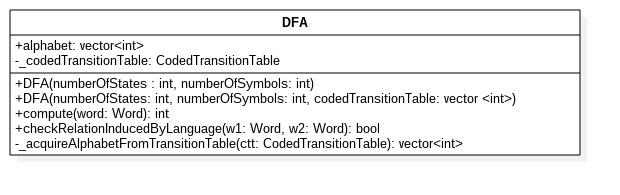
\includegraphics[width=0.4\textwidth]{images/dfa.jpg}
    \caption{Class diagram of Deterministic Finite Automaton}
    \label{fig:dfa_class}
\end{figure}



%---------------------------------------------------------------
%---------------------------------------------------------------

\subsection{Math}

The math module shown in figure~\ref{fig:math_class} should contains all necessary classes from mathematical computations. The class \textit{Point} encapsulates a point in d dimensions. Such point can be instantiated with any type.

%
% MATH CLASS DIAGRAM
%
\begin{figure}[H]
	\centering
	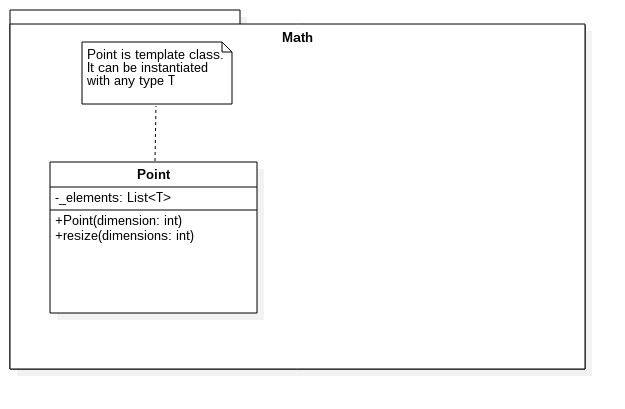
\includegraphics[width=0.45\textwidth]{images/math_class.jpg}
    \caption{Class diagrams of math module}
    \label{fig:math_class}
\end{figure}




%
% WORD PROCESSING CLASS DIAGRAM
%

\subsection{Words Processing}
To perform words generation/processing we will use classes presented on figure \ref{fig:words_processing_class}.

Since it happens to be largest and most important of all four, let us first focus on \texttt{WordsGenerator} class. Its main purpose is to create words using rules described in methodology  . There are in fact two type of conditions to cover:
\begin{itemize}
\item parametrical, where the class checks global parameters related to word processing
\item hamming condition, generated word of some length, let us say $n$, must have hamming distance between all (up to now) generated words of length $n$ smaller than some defined constant.
\end{itemize}

Check of the first one is done via \texttt{\_checkGlobalConsitions()} and latter one is covered by \texttt{\_hammingCondition()}. As one can easily see, \texttt{\_hammingDistance()} method is just an auxiliary procedure for work related to checking hamming condition. Although method \texttt{\_generateRandomWordOverAlphabet} speaks for itself, \texttt{\_generateRandomWordStartinWith} needs some explanation. As we are forced to firstly produce words starting with different symbols of alphabet, this method provides a way to create such a word with hamming condition checked. User specifies only starting symbol and length of the word and procedure returns random word starting with particular symbol and of specified length. There are only two public methods: constructor, which forces user to specify alphabet and \texttt{getPairs()}. The last one's ability is to gather all generated words and combine them into pairs. Such approach is forced by PSO's fitness function. 

Despites its vague name, \texttt{BagOfWords} is class which preserves set of words in form of an unordered map, where keys are lengths and entries are vectors of words of specified length. It enables easy access to words of some particular length. We took such approach because most comparisions in the \texttt{WordsGenerator} class is done by checking hamming condition, which concerns words of the same length. What is more methodology obliged us to create 3 disjunctive sets of words: $\Omega_S$, $\Omega_M$ and $\Omega_L$ and using this class we can fulfil this need, preserving all desired functionality. When needed one can always gather all words as a vector using \texttt{getAllWords()} method.

Last two classes were created to make code more transparent. \texttt{PairOfWords} simply wraps two words together and \texttt{Word} class supplies user with short set of methods operating on vector of integers (which simulates a word). As mentioned they are more needed because their names than actual functionalites.

\begin{figure}[H]
	\centering
	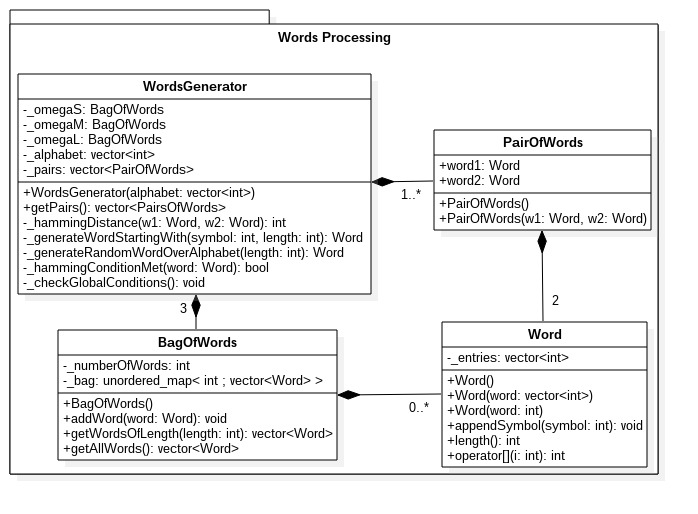
\includegraphics[width=0.4\textwidth]{images/words_processing.jpg}
    \caption{Class diagram of words processing clases.}
    \label{fig:words_processing_class}
\end{figure}

%
% TRANSITION TABLE CLASS DIAGRAM
%
\subsection{Transition Table}
Classes used to model behaviour of transition table are presented on figure \ref{fig:trans_table_class}. 

\textcolor{red}{Remark:} It is worth to notice that in all consecutive classes, entries of transition tables stays as a vector of integers. Each table, beginning with \texttt{StandardTransitionTable}, provides its own way to read values from the vector either via overloading \texttt{operator ()} or by implementing methods.

As one can see, starting from most general \texttt{TransitionTable} and going up on chains of inheritance classes broad they abilities. Base class provides only methods for loading automaton from file specified via \texttt{url} string. It is able to either load it symbol by symbol ( \texttt{\_loadOneSymbol()} ) or fill up all entries at once - \texttt{\_loadEntries()}. Entries at this level can not be interpreted using any transition table type - it is just raw data.

Next, one can create \texttt{StandardTransitionTable}, which interprets \texttt{\_entries} as a table where columns represents symbols and rows are states. Classes, which will inherit from this one are provided with method \texttt{\_accessTransitionTable()} and for public usage \texttt{operator ()} has been overloaded. Both approaches force to pass symbol and state and as a results guarantee state. 

Thrid  is \texttt{PerSymbolTransitionTable}, which is more suited for computer interpretation of automaton. It assumes that each symbol has its own table. Each table's column and rows represents consecutive states and entries takes values equal to either $0$ or $1$. Such a values describe situation when "two states are not connected" and "there is connection between states", repsectively. Simmiraly to \texttt{StandardTransitionTable}, there are two ways to acces table. Public access is provided by overloaded \texttt{operator ()} and protected access is anabled via \texttt{\_isTransition()} method. Both needs two states and symbol to determine whether there is connection or not, hence return value is of boolean type.

Last but not least, we have \texttt{CodedTransitionTable} class. First observable difference appears in constructors - this class enables to initialize transition table either via loading and coding automaton from file or accepting coded automaton and decoding it to achieve transition table. Such approach has been forced by Particle Swarm Optimization algorithm. TO be a little bit more precise: paticles are represented by coded deterministic finite automata and need to be updated, which causes automata to change. In such a case we just create new automaton from updated particle's coded DFA table. \texttt{\_getCodedTransitionTable}, as name says, returns coded table, which then can be used as a position of particle within PSO space.




\begin{figure}[H]
	\centering
	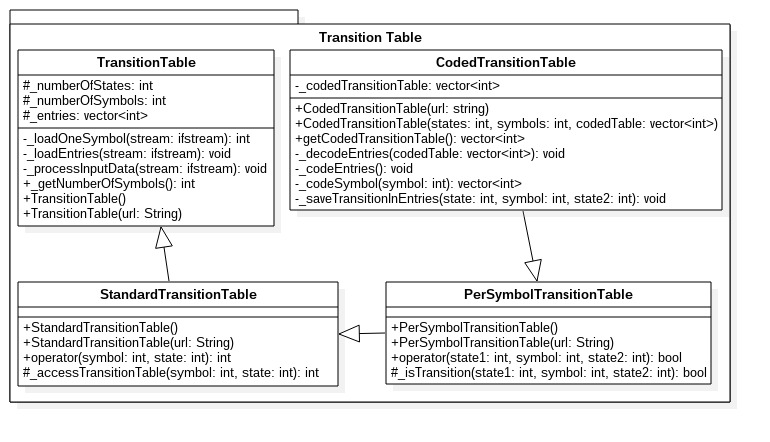
\includegraphics[width=0.4\textwidth]{images/transition_table.jpg}
    \caption{Class diagram of classes implementing different transition tables notations.}
    \label{fig:trans_table_class}
\end{figure}



\end{document}
